\documentclass{cce2014-design}
\svnInfo $Id: design_brief.tex 8578 2024-05-21 18:32:00Z gcar0029 $

\usepackage{bookmark}
\usepackage{geometry}
\geometry{headheight=15pt}
\usepackage{amsmath}
\usepackage{graphicx}
\usepackage{verbatim}
\usepackage{float}
% Document details
\title{Design Brief: Group 03}
\author
{
	Gabriel Carabott,
	Gioele Giunta,
	Jacob Ellul
}
\date{\svnMaxToday, Document v.\svnInfoMaxRevision}

\begin{document}

\maketitle

\begin{abstract}
	The system described processes DTMF signals from
	digital audio sources
	to display corresponding characters on an LCD display. Upon startup,
	users
	calibrate the system using a joystick, centering a * on
	the LCD.
	In reading mode, the system detects and displays DTMF tones. Users can
	select
	processing algorithms (Goertzel or FFT) via a dedicated settings page,
	with the
	choice indicated by an LED colour code. The LCD supports
	automatic-forward-scrolling for character display, with manual
	navigation
	enabled through joystick use. This abstract provides an overview of the
	system's capabilities and usser interactions, facilitating intuitive
	digital
	signal processing.
\end{abstract}

\section{Introduction}
 % Write an introduction, explaining the purpose and background of this project.
 % Give a brief description of the system to be implemented.
 % References to be cited like so \cite{stroustrup2000}.
 % Also include an overview of this document.
 {
  DTMF signals	\cite{wikiDTMF} are an effective way of transmitting a small
  set of
  information over a noisy and bandwidth-constrained medium,
  with excellent decodability even in the worst of conditions. This also
  extends to telephony, where a proof of concept may be
  devised in absence of an active phone network or the approval of a
  service provider. Such an environment is where this project
  exists, a model for rudimentary communication over the phone line in
  the 21\textsuperscript{st} century.

  The ARM MDK was used as the primary testing environment for our code.
  The implementation uses
  various libraries/drivers provided by the MDK, Labs and occasionally github.
  Keil within a
  windows Operating system was the environment that was used mostly,
  furthermore Keil was also used to load data onto the board. However for
  developement and testing other environments were used for
  speed and easier testing of features that do not require the board(e.g.
  VSCode in WSL).
  All code was written in C using the C standard for naming and syntax
  for files, functions and variables.

  This document will go through each component of the system individually
  providing a full overview of the system we have created and how each
  component contributes to it.

  \begin{figure}[H]
	  \centering
	  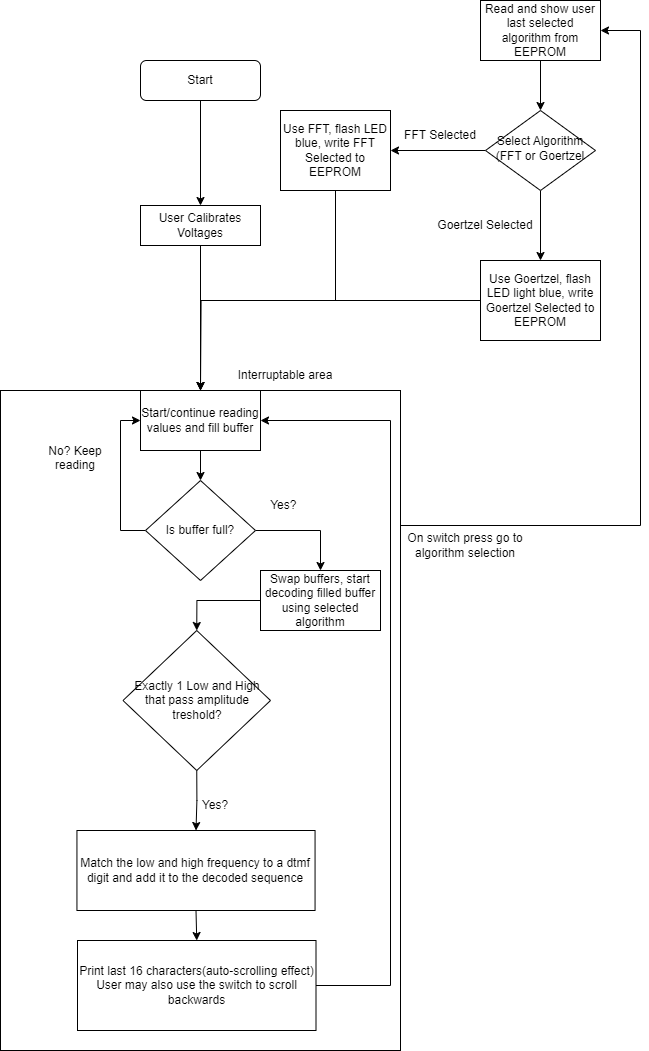
\includegraphics[width=0.5\textwidth]{sys_diagram}
	  \caption{System Overview Diagram}
	  \label{fig:systemDiagram}
  \end{figure}
 }

\section{System Design}
 {
  \subsection{Circuit}
  {
	  \textbf{Theory:}
	  The handbook's reference (Handbook's Figure 1) served as the
	  model for the circuit that was made, though some adjustments were
	  made to make
	  it more compatible with easily accessible components.
	  \begin{figure}[H]
		  \centering
		  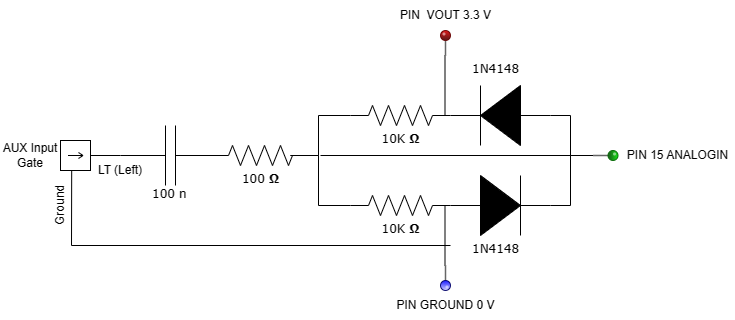
\includegraphics[width=0.5\textwidth]{circuit-diagram}
		  \caption{Circuit Diagram (Adapted)}
		  \label{fig:Circuit Diagram(Adapted)}
	  \end{figure}

	  The left channel of the AUX input is used as the input signal
	  for the circuit, and its ground is connected to the board's ground
	  (GROUND PIN
	  0V). The input signal is received through an AUX input socket.

	  The ground is linked to the GROUND 0V pin of the LPC4088 board,
	  and the upper input, which will act as the maximum voltage for the
	  output wave,
	  is obtained from the 3.3 V VOUT pin of the board. Next, the circuit's
	  output is
	  linked to the board's ANALOGIN PIN 15.

	  In this circuit, the 100Ω resistor and 100n capacitor placed
	  near the input form a low-pass filter to condition the input signal.
	  In
	  addition, the two 1N4148 diodes and 10kΩ resistors serve to move the
	  signal
	  upward, ensuring that it is fully positive before being sent to the
	  ADC.	This
	  is critical because if the input signal were to oscillate around 0V,
	  the part
	  of the signal that becomes negative would be interpreted as 0 by the
	  ADC,
	  resulting in incomplete and inaccurate readings.

	  \begin{figure}[H]
		  \centering
		  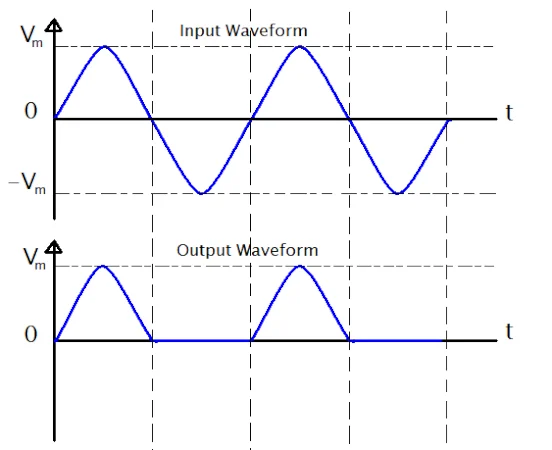
\includegraphics[width=0.5\textwidth]{ADC-problem}
		  \caption{ADC 0 Problem (Possible condition)}
		  \label{fig: ADC 0 Problem (Possible condition)}
	  \end{figure}

	  The ADC on the LPC4088 board, can read only positive values,
	  from 0V to VCC (in this case: 3.3V). Any negative portion of the
	  input signal
	  would be lost (Figure 3). For this reason, it is essential to
	  vertical shift
	  the
	  entire signal upward (Figure 4), thus avoiding signal loss, which
	  could disturb
	  signal
	  processing in the future.

	  \begin{figure}[H]
		  \centering
		  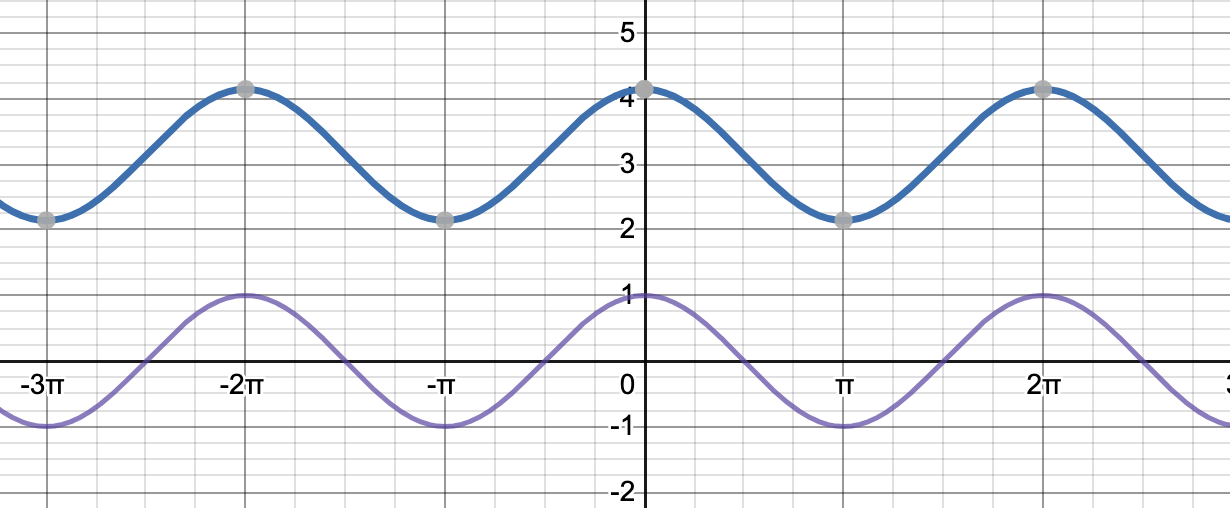
\includegraphics[width=0.5\textwidth]{shift-upward}
		  \caption{Shifting Signal Upward}
		  \label{fig: Shift Upward}
	  \end{figure}

	  \textbf{Implementation:}
	  The realization of the Circuit above (Figure 2), was done using
	  a breadboard.
	  Unlike the circuit depicted, the realization was done by
	  connecting the VOUT PIN 3.3 V to the positive line of the breadboard
	  (red), and
	  the GROUND PIN 0V to the negative line of the breadboard (blue).

	  The 1N4148 diode and 10k ohms resistor connected to the
	  positive line with one lead, with the other terminal both were
	  connected to
	  horizontal line number 15 of the breadboard.

	  In line number 15 of the breadboard, the terminals of diode
	  1N4148 and 10k ohms resistor connected with a lead to the negative
	  line were
	  also inserted.

	  Finally, in line 15 the lead of the 100 ohms resistor was also
	  connected. And PIN 15 was also connected to line 15.

	  This architecture allowed a lower probability of errors
	  determined by faulty leads or failed breadboard leads.

  }
  \subsection{Reading}
  {
	  \textbf{Introduction:}
	  One of the most important parts of the system is the analog
	  data collection module, which records and stores analog signals at a
	  particular
	  sampling rate. The main application will receive a constant stream of
	  data from
	  this module for further processing and analysis.

	  \textbf{Sampling Rate Considerations:}
	  The module is designed to operate at a sampling rate of 8000 Hz
	  (SAMPLE\_RATE), as defined in the code:

	  In choosing this sampling frequency, the Nyquist-Shannon
	  theorem is carefully followed, according to which the sampling
	  frequency must
	  be at least twice the highest frequency contained in the signal. The
	  highest
	  frequency component in Dual-Tone Multi-Frequency (DTMF) signaling is
	  1633 Hz.
	  By setting the sampling frequency to 8000 Hz, high frequencies that
	  may contain
	  transients are captured and the aliasing effect on frequencies above
	  2 kHz is
	  avoided. In this way, the captured signal will contain enough
	  information to
	  accurately reconstruct the original signal.
	  \begin{equation}
		  8000 > 2 \cdot 1633
	  \end{equation}

	  \textbf{Array Size and Sampling Window:}
	  The size of the arrays (main\_array and secondary\_array) is
	  set to 512 elements (ARRAY\_ELEMENTS). This was chosen because it is
	  a power of
	  2, which is an important detail for running the FFT for the signal
	  processing
	  stage. The size of 512 elements, also proved to be optimal through
	  experiments
	  in MATLAB that revealed that a sampling window of 0.064 seconds,
	  obtained with
	  an array size of 512 elements and a sampling rate of 8000 Hz, is
	  sufficient to
	  capture all the frequency components present in DTMF signals, as
	  verified using
	  Audacity (Figure 5).
	  \begin{figure}[H]
		  \centering
		  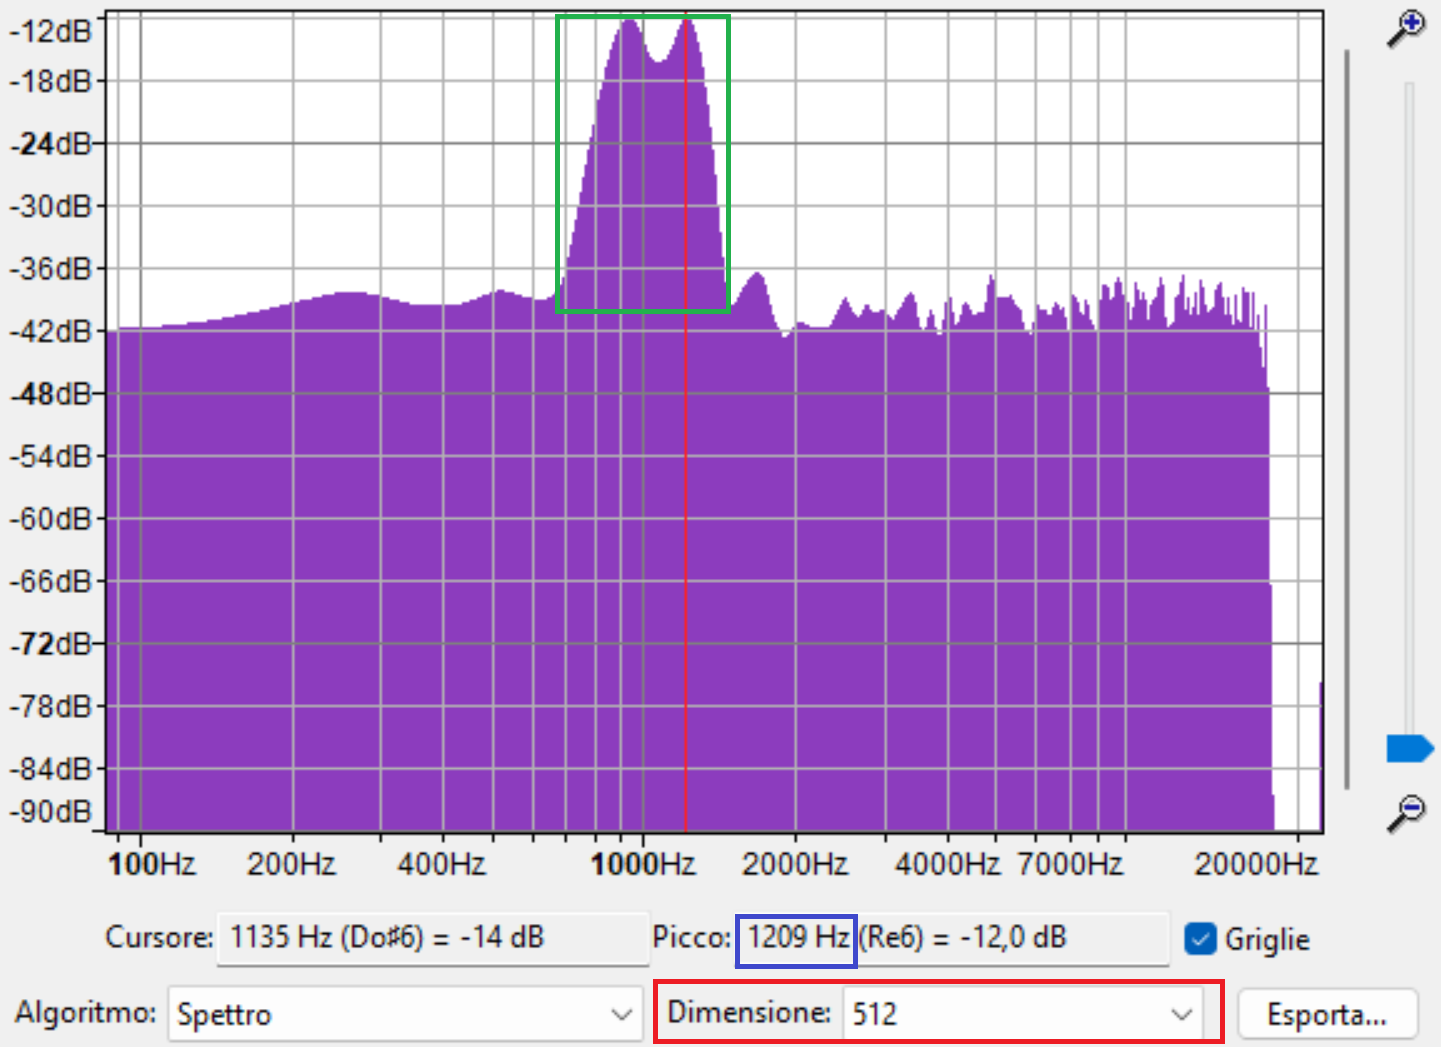
\includegraphics[width=0.5\textwidth]{spectrum-window}
		  \caption{Audacity Output Spectrum}
		  \label{fig: Spectrum (Window Size: 0.064s, Sampling Rate:
			  8000Hz)}
	  \end{figure}

	  \textbf{Analog Data Acquisition:}
	  Analog data is read from the module by the ADC, which reads from
	  PIN 15 of the ANALOGIN area of the board the voltage level
	  provided by the Circuit (Circuit Section).
	  The read() function uses two arrays,
	  main\_array and secondary\_array, to construct a circular buffer
	  in which the analog value is read from the ADC and stored.
	  The system utilizes a SysTick configured at the 8000 Hz sampling
	  frequency to generate an interrupt that calls the read() function,
	  enabling the acquisition of analog data at this rate.

	  \textbf{Double-Buffering Technique:}
	  The module employs a double-buffering technique to ensure
	  continuous data acquisition without interruption and without losing
	  any part of
	  the signal. When one array is full (counter >= ARRAY\_ELEMENTS), the
	  data\_ready flag is set to indicate that a new array is available for
	  processing, and the array\_ready pointer is updated to point to the
	  recently
	  filled array. The module then swaps the current\_data pointer to the
	  other
	  array and resets the counter, allowing the acquisition process to
	  continue
	  seamlessly. This is observed in Figure 6.

	  \begin{figure}[H]
		  \centering

		  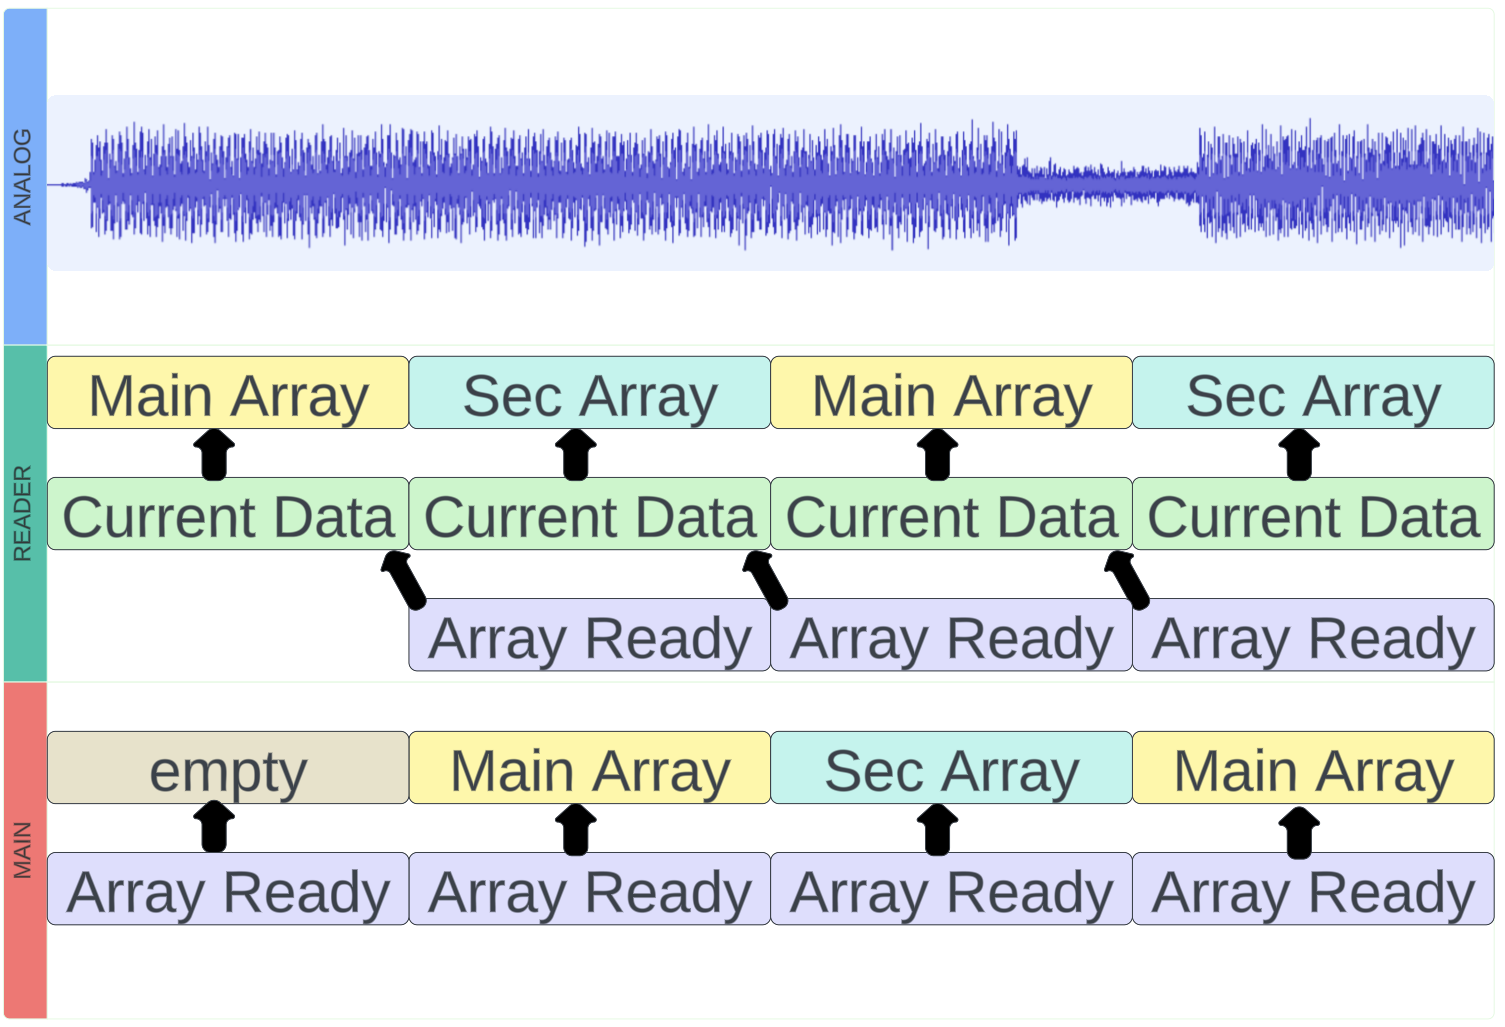
\includegraphics[width=0.5\textwidth]{circular-buffering}
		  \caption{Circular Buffering Mechanism}
		  \label{fig : Circular Buffering}
	  \end{figure}

	  \textbf{Calibration and User Interface:}
	  The module manages the initialization and configuration of the
	  calibration settings for the analog mask. The details of the
	  calibration
	  process and user interface will be covered in the "User Interface"
	  section.

	  \textbf{Performance Measurements:}
	  Measurements of the program's modules, including the SysTick, have shown that the reading and saving operations have a low time cost.
	  Specifically, it takes exactly 512 SysTicks to fill the array, indicating that the majority of the time is spent on the 512 ticks required to populate the array, while the reading ADC and saving operations contribute minimally to the overall time.
	  Since each Systick is equal to $\frac{1}{8000}$ s, the reader thus requires 64 ms to read the input.

	  \textbf{Shared Variables and Interfaces:}
	  The module exposes several global variables that can be
	  accessed by the main program. The data\_ready flag indicates when a
	  new array
	  of data is available for processing by the main program, while the
	  array\_ready
	  pointer provides access to the most recently filled array. The
	  status\_flag
	  variable can be used to temporarily disable the reading process if
	  needed. In practice this was not used as both algorithms are faster
	  than the reader.
	  The calibrated flag indicates whether the analog mask has been
	  calibrated. If this flag is not set to true the reading and decoding
	  process will not start.
  }
  \subsection{Fast Fourier Transform}
  {
	  \subsubsection{FFT Testing and developement}
	  The FFT was developed using cooley-tukey's example
	  \cite{cooleyTukeyFFT}, first the
	  simple version was used and adapted for the board.
	  Then the more complex yet far more efficient version was
	  adapted for the board and tested. Both versions were tested in python
	  using a
	  few scripts:
	  \begin{enumerate}
		  \item audio.py: This script read a .wav file (tested
		        with DTMF tones) and filled a text file with the values
		        read ranging from -1000
		        to 1000 for the first tone detected. Additionally the
		        wave is plotted to ensure the values are correct
		        (Figure 7)
		        \begin{figure}[H]
			        \centering
			        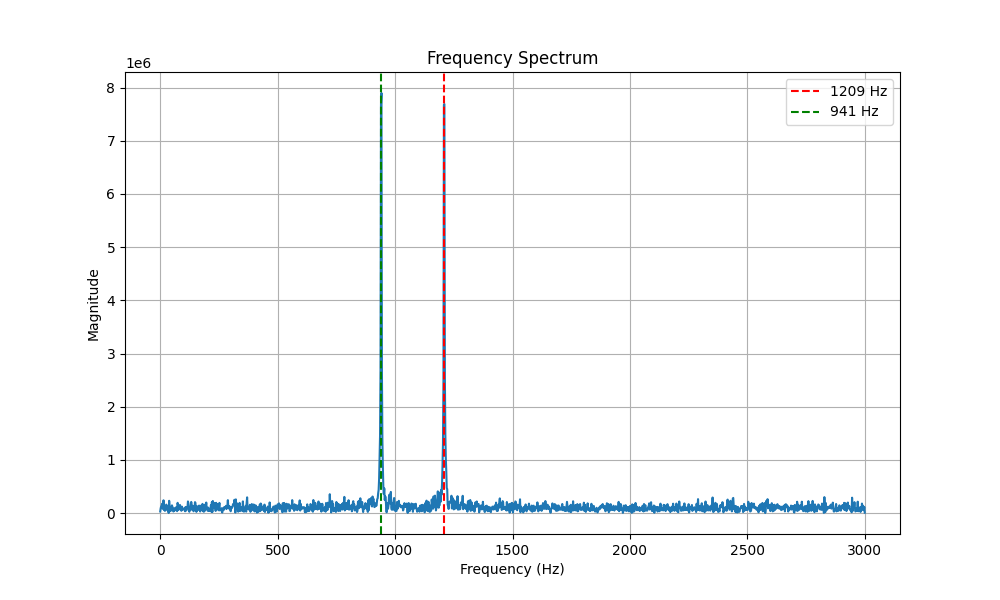
\includegraphics[width=0.5\textwidth]{spectrum}
			        \caption{Example Input Plotted as a
				        Spectrum (*)}
			        \label{fig : Example Input Plotted as a
				        Spectrum}
		        \end{figure}
		  \item plots.py: This script was used to plot the FFT
		        output of the C code to ensure that it is working
		        correctly. (Figure 8)
		        \begin{figure}[H]
			        \centering
			        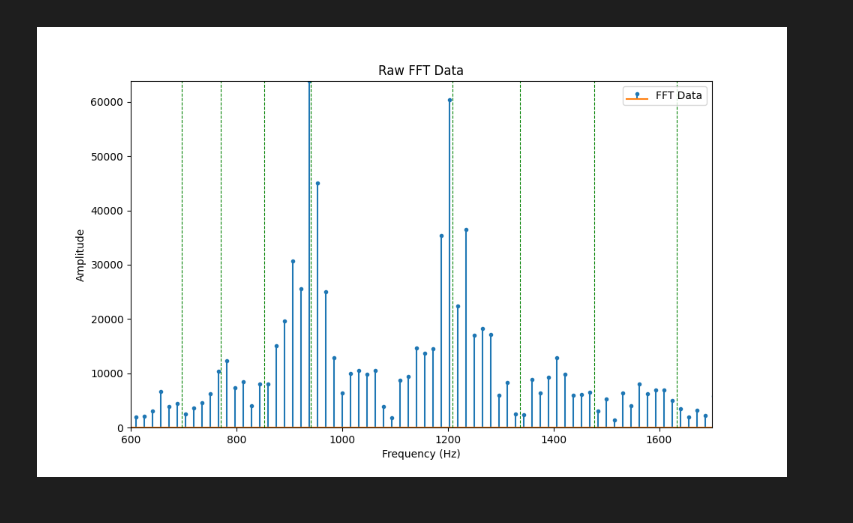
\includegraphics[width=0.5\textwidth]{fft}
			        \caption{ Plotted Example Output
				        Produced by the FFT (*)}
			        \label{fig : Plotted Example Output
				        Produced by the FFT}
		        \end{figure}
	  \end{enumerate}

	  With these scripts the FFT was tested and verified to be
	  working correctly. The FFT was then integrated into the system and
	  tested with
	  the DTMF tones on the board.

	  \subsubsection{Decoder}
	  The decoder then gets the FFT output and checks the frequences
	  we care about and calculates their amplitudes (with a margin as the
	  frequencies
	  aren't always exactly what they should be, ex: 697 Hz could be 703.4
	  Hz).
	  It does this for both the high and low frequencies and then
	  sends the results to the comparator. If there is exactly 1 high and 1
	  low then
	  it sends the matching frequencies to the comparator. Otherwise if
	  there are
	  more than
	  1 high and low (ex. 2 high 2 low). Then the decoder will send
	  an error message to the comparator. The splitting of the decoder and
	  comparator
	  was done to break up the responsability of
	  matching a frequency to a character and indicating error
	  messages to the user (comparator) vs decoding the fft output
	  (decoder). For timing purposes the final FFT was measured at 412 ticks, which translates to 52 ms.
	  Initially this was tested by printing the output of the
	  decoder and checking that it matches what we are expecting. This was
	  then
	  substituted to return the values to the comparator.
  }
  \subsection{Goertzel Algorithm}
  
	This approach calculates the magnitudes of the DTMF frequencies and determines the dominant frequencies for decoding in a DTMF compliant signal.
	In the program, these steps are performed separately in distinct functions.
	Furthermore, this implementation does not utilise any external mathematics libraries, improving its portability and, most importantly, making it exceptionally fast, even on constrained hardware like the board of this project.
	Lastly, in order to highlight actual frequencies and attenuate noise, the magnitude squared is returned as the amplitude, which also eliminates additional calculations since the defined algorithm already finds the magnitude squared immediately.

	A major contribution to this implementation was the article on the algorithm published by \textit{embedded.com}, which explains the theory behind the algorithm, a base for how it may be devised as well as example runs. \cite{gtzl-embedded}

	\subsubsection{Implementation}

		The first component determines amplitudes of DTMF frequencies from an array of voltage level samples of the input signal.

		Despite the input array containing 512 elements, only 508 are used, in order to have Goertzel frequency buckets which match the DTMF frequencies as much as possible.
		This was decided after using the following equation to get an index, $i$, closest to an integer, where the input array size, $s_a$, was the variable:
		\begin{align*}
			i = \frac{f}{f_s \div s_a}
		\end{align*}
		The average, taking each value of $s_a$, was approximately equal to 508 thus, it was used.

		Although hidden from the user, constants are computed before the first call to the function to lighten its load, leading to lower execution times.
		These are computed as follows, where $f_s$ is the sampling frequency:
		\begin{itemize}
			\item{$k_f = \frac{(\text{INPUT\_ARRAY\_SIZE}) \cdot f}{f_s}$}
			\item{$w_f = \frac{2 \pi}{\text{INPUT\_ARRAY\_SIZE}} \cdot k_f$}
			\item{$\text{sin}_f = \sin{(w_f)}$}
			\item{$\text{cos}_f = \cos{(w_f)}$}
			\item{$\text{coeff}_f = 2 \cdot \text{cos}_f$}
		\end{itemize}

		Computation occurs over each element of the input array, where the focus is on the three following variables:
		\begin{itemize}
			\item{$Q_0$: the current value}
			\item{$Q_1$: the previous value -- the value of $Q_0$ one iteration ago}
			\item{$Q_2$: the value of $Q_0$ two iterations ago}
		\end{itemize}

		The amplitude function concludes with the calculation of the magnitude squared, which is performed as follows for each applicable frequency:
		\begin{align*}
			\text{Magnitude}^2 = (Q_1)^2 + (Q_2)^2 - (Q_1 \cdot Q_2 \cdot \text{coeff})
		\end{align*}
		Each amplitude is saved in an array given to the function as an argument, which is obviously defined outside of the function and thus, may be used in other functions.

		The other component involves taking the aforementioned amplitudes and determining the dominant frequencies in the signal while checking that the input is DTMF-compliant.
		The function goes through each frequency, dealing with low and high frequencies separately yet simulatenously, and checks if the matching amplitude exceeds a certain threshold, one which was determined after rigorous testing.
		Furthermore, if more than a single low or high frequency exceeds the threshold, the signal is no longer DTMF compliant and therefore, the function ceases execution and returns appropriately to indicate an error.

	\subsubsection{Performance}

		When testing the functions in an early version of the program, this implementation of the algorithm performed excellently, both in terms of speed and reliability: tones were decoded almost immediately as they started, which also proves the superb quality of other program units further along the pipeline, while also detecting when more than one DTMF tone was played at a given time.

		With regards to its capability to decode through noise, the implementation also surpassed expectations, even able to extract the correct frequencies when, using specially crafted audio files, the signal-to-noise ratio was only 50\%, when the signal had a low amplitude and even a combination of the two.

		Most importantly, both functions calls return before a window of samples is read from the input signal, resulting in a system that samples the input perfectly without dropouts.
		To measure execution time, another version of the program measured the amount of ticks taken to execute both functions, where each tick is equal to $\frac{1}{8000}$ seconds.
		Through lengthy experimentation, they were determined to take approximately 15 ms, four times as fast as the reader.
		Hence, it is same to assume that decoding will never inhibit reading.

	\subsubsection{Example}

		This example contains a hash character, defined in the DTMF by the frequencies 941 and 1477 Hz, mixed with white noise at a ratio of 1:3 (signal:noise), displayed spectrally in Figure \ref{subsub:gtzl-eg-hash-spectrum}.
		\begin{figure}[H]
			\centering
			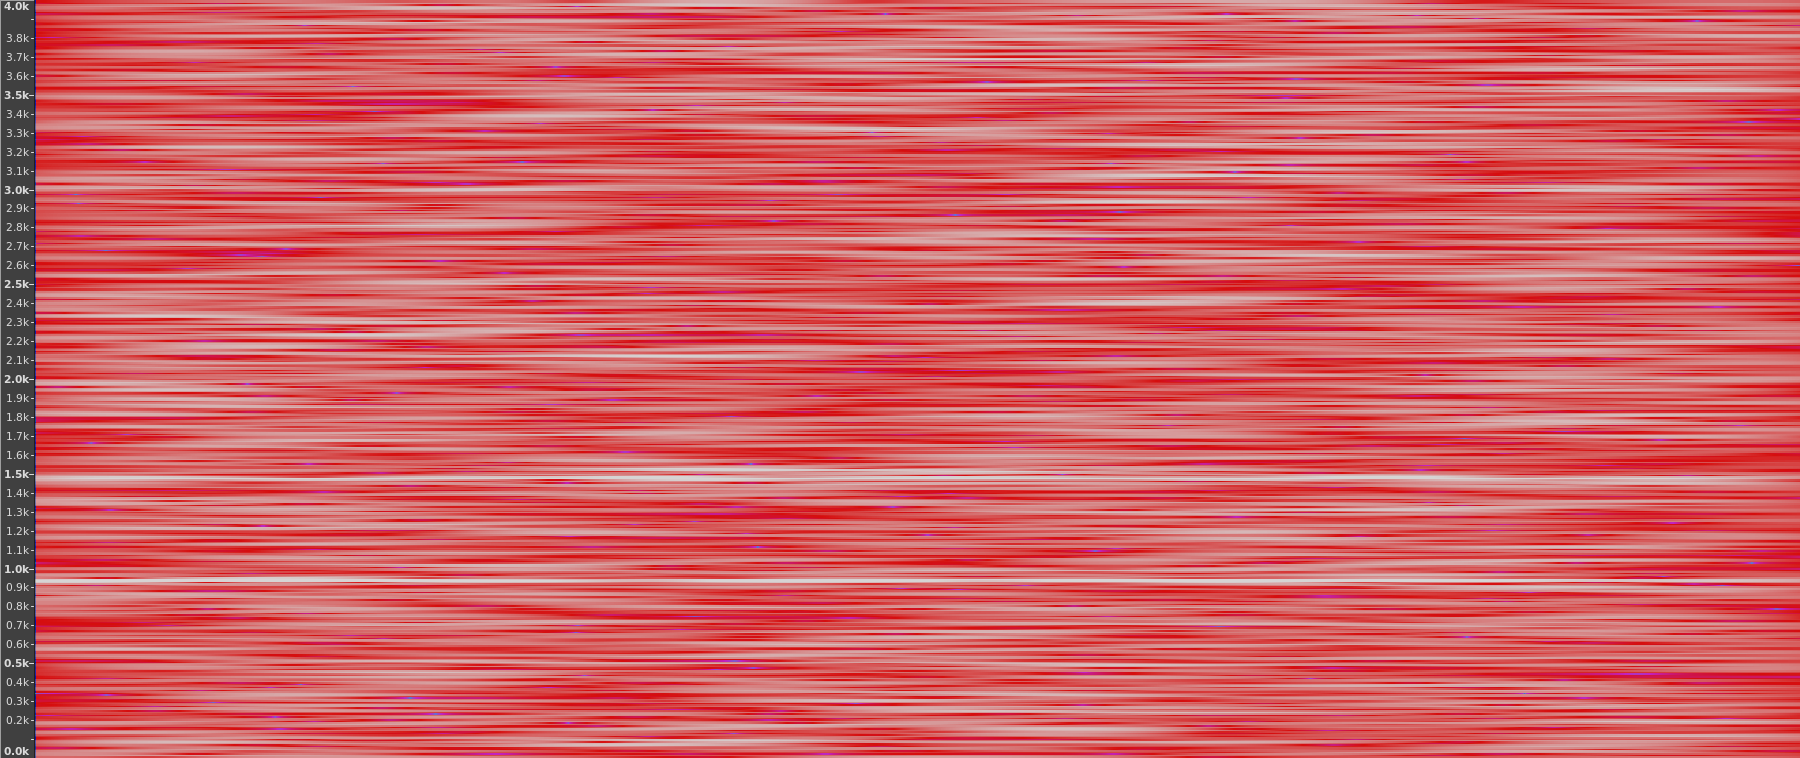
\includegraphics[width=\linewidth]{hashDTMF-75N25S-8000FS-spectrum.png}
			\caption{The spectral representation of a hash character in DTMF mixed with white noise}
			\label{subsub:gtzl-eg-hash-spectrum}
		\end{figure}

		After passing the audio file to the Goertzel functions, the amplitudes for each frequency were presented, neatly plotted in Figure \ref{subsub:gtzl-eg-hash-chart}.
		\begin{figure}[H]
			\centering
			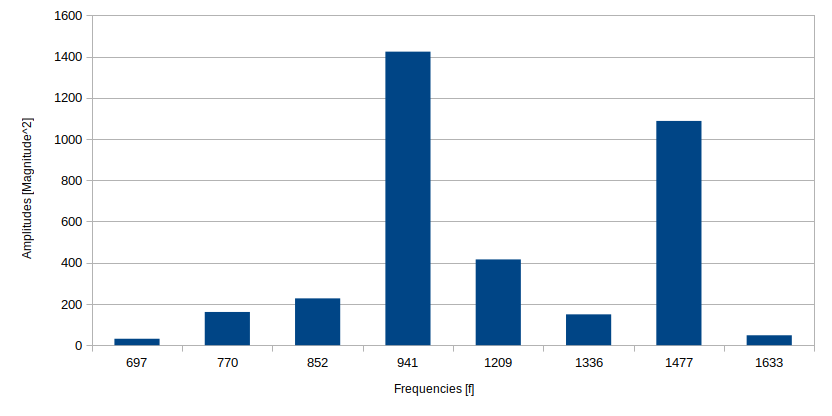
\includegraphics[width=\linewidth]{hashDTMF-75N25S-8000FS-chart.png}
			\caption{Graph of amplitude vs. frequencies for the DTMF hash mixed with noise}
			\label{subsub:gtzl-eg-hash-chart}
		\end{figure}
		Furthermore, the dominant frequencies identified were 941 and 1477 Hz.
		If the amplitude threshold is taken to be 800 for this prototype, this illustrates that the correct frequencies were identified and that the signal was found to be DTMF compliant, despite the noise present.

  \subsection{Frequencies Comparator}
  {
	  \textbf{Introduction:}
	  The tone\_frequencies structure, which contains high and low
	  frequency values from the input signal, is sent to the
	  frequencies\_comparator
	  module by the decoding area. The primary function,
	  frequencies\_comparator,
	  determines the associated key by comparing these frequencies with the
	  DTMF
	  matrix. This module can recognize and manage various error
	  situations,
	  distinguishing between situations where there is no DTMF signal
	  detected (both
	  high and low frequencies are zero) and those in which several DTMF
	  signals are
	  detected at once (high or low frequency is -1). In these cases, the
	  module
	  returns the appropriate error code and sets the last\_char to 'N'
	  (noise).

	  \subsubsection{Duplicate Key Prevention and Sequence Management:}
	  The module also prevents duplicate keys from being added to the
	  character sequence by comparing the recognized key with the
	  last\_char. If they
	  differ, the add\_char\_to\_sequence function is used to append the
	  identified
	  key to the sequence and set the last\_char to the actual key. This
	  function
	  looks also for possible overflow situations. Both in this case and in
	  MultiTone
	  detect, the module takes advantage of the global variables provided
	  by the
	  errorm file, setting an error text, as will be seen in the 'Error
	  Handling'
	  section.

	  \subsubsection{DTMF Matrix and Key Recognition:}
	  The recognized key is the value obtained from the DTMF matrix
	  based on the row and column indices corresponding to the high and low
	  input
	  frequencies. The algorithm sets last\_char to "N" when the
	  lower\_frequency and
	  higher\_frequency comparison functions return -1.

	  \subsubsection{Frequency Comparison Functions:}
	  The comparison functions play the role of associating a column
	  from 0 to 3 or -1 with a higher\_Frequency, and a row from 0 to 3 or
	  -1 with a
	  lower\_Frequency.

	  \begin{figure}[H]
		  \centering
		  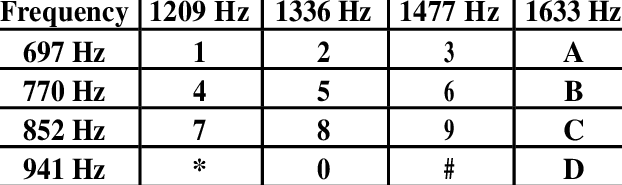
\includegraphics[width=0.5\textwidth]{tone-table}
		  \caption{DTMF Matrix}
		  \label{fig: DTMF Matrix}
	  \end{figure}
	  These assembly functions exploit the CMP->ITT logic
	  studied
	  in the Arm Documentation \cite{armDocumentation}, for the creation of
	  a switch case, in order
	  to avoid
	  the classic jump structure in assembly.

	  \subsubsection{Overview:}
	  The 0.064-second sampling window allows the system to pick up
	  even the smallest bits of noise or stillness.
	  Because of the extremely small sample window, the algorithm can
	  identify that consecutive 1s are part of an analysis of the same tone
	  if it
	  comes across a sequence like (1, 1, 1, 1, 1, Noise, Noise, 1, 1, 1,
	  Noise, 2,
	  2, 2, 2, 2, 3, 3, 3). On the other hand, last\_char is set to "N"
	  when noise is
	  detected, enabling the system to recognize the subsequent 1s sequence
	  as a new
	  tone.
	  As a result, (1,1,2,3) would be the character sequence that was
	  read by the main program and stored in the 'sequence' array.

	  \subsubsection{Timing Measurements:}
	  Measurements using systick\_Counter, a counter that increments
	  by 1 on every systick interrupt, have shown that the time required
	  for the
	  frequencies\_comparator module is 63 ticks, equal to 8 ms.
  }

  \subsection{User Interface}
  {
	  Both mask\_calibrate.c and algorithm\_setter.c share a common
	  user interface through LCD and joystick controls.
	  However, their specific implementations and purposes
	  are different.

	  \subsubsection{Common Title Scrolling}
	  The modules implement a scrolling mechanism to display
	  instructions on the top line of the LCD screen.
	  The difference is that since the mask\_calibrate is
	  called by the read 8000 times per second the scrolling
	  takes place via systick\_counter, while instead the
	  algorithm\_setter which is called once by the interrupt of
	  the user button implements a while loop.

	  \subsubsection{mask\_calibrate.c}
	  The file mask\_calibrate.c contains functions to calibrate
	  the mask value, which is essential for accurate signal
	  processing. The read function in Reader.c calls the main
	  function mask\_calibrate 8000 times a second when the
	  system is not yet calibrated.

	  \subsubsection{Calculation of the mask value}
	  The calculation of the mask value is performed
	  using the following expression:
	  \begin{equation}
		  \text{mask\_value} = \frac{\text{max\_amplitude} \times
			  \text{res}}{\text{half\_amplitude} \times
			  \text{vadc}}
	  \end{equation}
	  This expression is the inverse of the output value
	  obtained from the read function in Reader.c and is
	  calculated as follows:
	  \begin{equation}
		  \text{vadc} = \frac{\text{res} \times
			  \text{max\_amplitude}}{\text{ADC\_MASK}} -
		  \text{half\_amplitude}
	  \end{equation}
	  By inverting the expression, the mask\_calibrate function
	  can determine the mask value based on the PIN 15 (ANALOGIN) Output.
	  For this
	  reason it is important to not play audio during the calibration stage
	  as it
	  will result in the mask value being incorrect and the (*) seemingly
	  jittering across the
	  bottom row of the screen. For a truly accurate reading just do not
	  play audio while calibrating.

	  \subsubsection{Graphic representation}
	  The show\_mask\_settings function uses a switch case
	  to identify the appropriate level range for the current
	  mask value and displays a star (*) at the appropriate
	  location on the bottom line of the LCD. Interestingly,
	  higher mask values (above 300 or under -300) indicate
	  almost perfect centering of the mask, consequently the
	  star appears more centered.

	  \subsubsection{Joystick input}
	  At the joystick button press SW\_CR, the function sets
	  the calibrated flag to 1, indicating a successful
	  calibration, and clears the LCD screen.

	  \subsubsection{algorithmz\_setter.c}
	  The algorithm\_setter.c file provides a function to select
	  the decoding algorithm between the fast Fourier transform
	  (FFT) and the Goertzel algorithm. The main program calls
	  the algorithm\_setter function, probably in response to a
	  user key interrupt.

	  \subsubsection{Algorithm Selection}
	  The algorithm\_setter function displays the available decode
	  algorithm settings (FFT and GTZL) on the bottom line of the
	  LCD and allows the user to toggle between them using the
	  left and right joystick buttons. The currently selected
	  option is highlighted between two vertical bars (|).

	  \subsubsection{Joystick input}
	  At the joystick button press SW\_CR, the function returns
	  the selected algorithm (2 for FFT or 3 for GTZL) to the
	  main program. The main program can then store the selected
	  algorithm in EEPROM for later use.
  }
  \subsection{Display I/O}
  {
	  The I/O used in this project were a button and joystick, an LCD
	  display, and an LED.

	  \subsubsection{LED}
	  The LED is used to indicate which algorithm is currently selected.
	  The LED will be blue if the FFT algorithm is selected and light blue
	  if the Goertzel algorithm is selected or if it is in Settings
	  Mode (Green).

	  \subsubsection{LCD Display}
	  The LCD display is used to display the decoded characters to
	  the user. The LCD display is a 16x2 display, which means it can
	  display 16
	  characters on 2 rows.
	  The LCD display is also used to display the calibrator and the
	  algorithm selection screen. While in the reading/decoding stage the
	  top row is
	  used to print
	  the sequence of DTMF tones and the bottom row is used to
	  indicate error conditions to the user. To display more than 16
	  characters in
	  the top row, the display
	  automatically prints the last 16 characters in the buffer
	  giving the effect of `scrolling'.

	  \subsubsection{Joystick and Button}
	  The joystick is used for general purpose operations such as
	  scrolling back on the LCD display, selecting the algorithm and
	  calbrating the system. In scrolling the lcd and setting the mask
	  calibrator the joystick is polled
	  every 333ms. In setting the algorithm
	  the joystick is polled in a continuous while loop.
	  The use of the joystick in the mask calibrator is to confirm the
	  selection of the mask value.

	  The `user' button is used as a hardware interrupt to go back to the
	  algorithm selector screen from the reading/decoding screen.
  }
  \subsection{EEPROM}
  {
	  \subsubsection{Challenges}
	  Initially flash memory was being worked on to store the last
	  algorithm
	  selected. However, due to the complexity
	  of the flash memory and the time constraints, it was decided to use
	  the
	  EEPROM instead.
	  \subsubsection{Implementation}
	  We accomplished this using the help of a github page
	  \cite{githubEEPROM}
	  for an older board and adapted it to our board. There were some minor
	  fixes we had to change for the
	  githube code to work (issues with header files), but after changing
	  this it worked as expected.
	  The EEPROM is used to store the last algorithm selected by the user.
	  This was done by writing
	  the algorithm selected to the EEPROM
	  and then reading it on startup. The EEPROM was tested using a simple
	  program that wrote a value to the EEPROM
	  and then read it back. This was done to ensure that the EEPROM was
	  working correctly and that the values were
	  being stored and read correctly. The EEPROM was then integrated into
	  the system and tested with the full system for proper integration.
  }
 }

\section{Management}
 % Include a time plan.
 % Show task dependencies.
 % How are these going to be managed?
 {
  \subsection{Software Components}
  {
	  Under src all the code is present, drivers are contained in a
	  seperate directory named `drivers'. Each file has one responsability,
	  for
	  example decoder.c/h
	  are only responsable for decoding and simplifying the output of the
	  fft for the frequencies comparator. The coding style adapted was the
	  C
	  standard.
	  Header files contain all the includes necessary and the corresponding
	  c file only includes the header file. This was done to ensure that
	  the code is
	  following a consitent standard. Global paramatars as a header file is
	  used to provide global access to shared variables to multiple source
	  and header
	  files.
  }

  \subsection{Project Dependencies}
  {
	  Most parts of the project were developed independently as other
	  dependencies could typically be mocked in python or in C.
	  For example the FFT was developed using a mock reader in python and a
	  mock decoder in python as well. This allowed for the FFT to be
	  developed and
	  tested independently of the reader and decoder. Then once a component
	  was deemed to be completed it would be integrated into the main
	  project and
	  tested further for compatability.
  }
  \subsection{Development Strategy}
  {
	  The agile development methodology was used.
	  Weekly meetings were held to discuss progress, issues and division of
	  work.
	  As is evidenced by our agendas and minutes these meetings were
	  instrumental
	  to our developement as we were able to re-focus our efforts into the
	  appropriate components. The next section describes our time plan
	  shows
	  our work done each sprint further showing our usage of this
	  developement strategy.
  }
  \subsection{Time Plan}
  {
	  \begin{enumerate}
		  \item \textbf{Sprint 1 (Development): 13th March - 10th
			        April}
		        \begin{itemize}
			        \item Printing to the screen was finished with
			              a side scrolling prototype.
			        \item All required components were obtained.
			        \item Reader including circuit mostly finished,
			              refinements needed.
			        \item Frequency comparator was started.
			        \item The decoder and FFT was started
		        \end{itemize}

		  \item \textbf{Sprint 2 (Prototype): 10th April - 1st
			        May}
		        \begin{itemize}
			        \item FFT and Decoder was finished
			        \item Voltage Calibrator was finished
			        \item Reader was refined and finished
			        \item Goertzel Algorithm was started
			        \item A uVision project was setup and
			              each component was integrated
			        \item A prototype was finished with the
			              system able to read voltages and output
			              the decoded result.
		        \end{itemize}

		  \item \textbf{Sprint 3 (Full Product): 1st - 15th May}
		        \begin{itemize}
			        \item Saving the algorithm selected to
			              EEPROM was finished
			        \item Adding a menu screen was finished
			        \item The goertzel algorithm was finished
			        \item Interrupts back to the menu
			              screen were facilitated by the physical
			              button
			        \item The full system was finished and
			              integrated. It was tested rigourously and
			              passed all testing.
		        \end{itemize}

		  \item \textbf{Sprint 4 (Final Submission): 15th - 24th
			        May}
		        \begin{itemize}
			        \item The full project is committed to
			              SVN, including documentation.
			        \item Short demo video has been produced and
			              finished.
		        \end{itemize}
	  \end{enumerate}
  }\subsection{Addressing Functional Requirements}
  {
	  \begin{enumerate}
		  \item \textbf{F.1 Continuous Sampling and Display:} The
		        reader consistently samples inputs, decodes them, and
		        displays the information
		        promptly. User interaction through the joystick to back
		        scroll yields
		        near-immediate responses.
		  \item \textbf{F.2 Physical Interaction:} Interaction
		        with the system, including the display and other
		        components, is facilitated
		        through the physical joystick and the button. The
		        button is used to go back to
		        the menu screen and the  joystick is used as general
		        purpose for multiple
		        functions.
		  \item \textbf{F.3 LED Indicators:} The LED used is to
		        indicate which algorithm is currently selected. The LED
		        will be blue if the FFT
		        algorithm is selected and light blue if the Goertzel
		        algorithm is selected. It
		        also indicates that the system is currently decoding
		        (Blue or Light Blue) or is
		        in Settings Mode (Green). It also indicates an error
		        status using the red LED.
		  \item \textbf{F.4 LCD Display Usage:} The decoded
		        string is presented to the user via the LCD display.
		        The LCD display is also
		        used in the calibrator and the algorithm selection
		        screen. Furthemore it is
		        used to indicate error conditions to the user such as a
		        buffer overflow or
		        multiple DTMF tones detected.
		  \item \textbf{F.5 System should always be in a
			        well-defined (and safe) state:} Powering on the
		        system there is no way to enter
		        an undefined or unsafe state. The system will always
		        start in the calibrator
		        and the user will have to calibrate before using it. On
		        hardware interrupts the
		        user is returned back to this stage.
		  \item \textbf{F.6 Storage for Configuration Settings:}
		        The previous algorithm selected is stored in memory.
		        This is used to select the
		        algorithm on startup. The system will always start with
		        the last selected
		        algorithm unless the user selects otherwise.
		  \item \textbf{F.7 Error Indication:} The bottom row of
		        the LCD is used to indicate error conditions to the
		        user. Such as buffer
		        overflow and multiple DTMF tones detected.
		  \item \textbf{F.8 Prevention of Undefined States:} The
		        system's design inherently prevents users from entering
		        undefined states.
	  \end{enumerate}
  }
 }
\bibliographystyle{ieeetr}
\bibliography{references}

\end{document}
